%%%%%%%%%%%%%%%%%%%%%%%%%%%%%%%%%%%%%%%%%
% Beamer Presentation
% LaTeX Template
% Version 1.0 (10/11/12)
%
% This template has been downloaded from:
% http://www.LaTeXTemplates.com
%
% License:
% CC BY-NC-SA 3.0 (http://creativecommons.org/licenses/by-nc-sa/3.0/)
%
%%%%%%%%%%%%%%%%%%%%%%%%%%%%%%%%%%%%%%%%%

%----------------------------------------------------------------------------------------
%	PACKAGES AND THEMES
%----------------------------------------------------------------------------------------
\documentclass{beamer}

\mode<presentation> {

% The Beamer class comes with a number of default slide themes
% which change the colors and layouts of slides. Below this is a list
% of all the themes, uncomment each in turn to see what they look like.

%\usetheme{default}
%\usetheme{AnnArbor}
%\usetheme{Antibes}
%\usetheme{Bergen}
%\usetheme{Berkeley}
%\usetheme{Berlin}
%\usetheme{Boadilla}
%\usetheme{CambridgeUS}
%\usetheme{Copenhagen}
%\usetheme{Darmstadt}
%\usetheme{Dresden}
%\usetheme{Frankfurt}
%\usetheme{Goettingen}
%\usetheme{Hannover}
%\usetheme{Ilmenau}
%\usetheme{JuanLesPins}
%\usetheme{Luebeck}
\usetheme{Madrid}
%\usetheme{Malmoe}
%\usetheme{Marburg}
%\usetheme{Montpellier}
%\usetheme{PaloAlto}
%\usetheme{Pittsburgh}
%\usetheme{Rochester}
%\usetheme{Singapore}
%\usetheme{Szeged}
%\usetheme{Warsaw}

% As well as themes, the Beamer class has a number of color themes
% for any slide theme. Uncomment each of these in turn to see how it
% changes the colors of your current slide theme.

%\usecolortheme{albatross}
%\usecolortheme{beaver}
%\usecolortheme{beetle}
%\usecolortheme{crane}
%\usecolortheme{dolphin}
%\usecolortheme{dove}
%\usecolortheme{fly}
%\usecolortheme{lily}
%\usecolortheme{orchid}
%\usecolortheme{rose}
%\usecolortheme{seagull}
%\usecolortheme{seahorse}
%\usecolortheme{whale}
%\usecolortheme{wolverine}

%\setbeamertemplate{footline} % To remove the footer line in all slides uncomment this line
%\setbeamertemplate{footline}[page number] % To replace the footer line in all slides with a simple slide count uncomment this line

%\setbeamertemplate{navigation symbols}{} % To remove the navigation symbols from the bottom of all slides uncomment this line
}
%----------------------------------------------------------------------------------------
\usepackage{graphicx} % Allows including images
\usepackage{booktabs} % Allows the use of \toprule, \midrule and \bottomrule in tables
\setbeamerfont{caption}{size=\scriptsize}
\usepackage{hyperref}
\usepackage{listings}
%----------------------------------------------------------------------------------------
%	TITLE PAGE
%----------------------------------------------------------------------------------------
\title[]{ROS Build System} % The short title appears at the bottom of every slide, the full title is only on the title page
%----------------------------------------------------------------------------------------
\author{ARRA / AR2A} % Your name
\institute % Your institution as it will appear on the bottom of every slide, may be shorthand to save space
{
\textbf{A}dvancements for \textbf{R}obotics in \textbf{R}escue \textbf{A}pplications
}
\date{\today} % Date, can be changed to a custom date
%----------------------------------------------------------------------------------------
\AtBeginSection{\frame{\sectionpage}}
%----------------------------------------------------------------------------------------
\begin{document}
%----------------------------------------------------------------------------------------
\begin{frame}
\titlepage
\end{frame}
%----------------------------------------------------------------------------------------
%----------------------------------------------------------------------------------------
\begin{frame}{Introduction -  ROS Packages}
 \textbf{Why ROS-Packages}
 \begin{itemize}
 \item Software in ROS is organized in packages
 \item It provides a way to easily reuse ROS-Software
 \end{itemize}
  \textbf{A ROS package might contain:}
 \begin{itemize}
 \item ROS nodes
 \item  a ROS-independent library
 \item a dataset
 \item configuration files
 \item a third-party piece of software
 \item or other useful modules that can be grouped together logically
 \end{itemize}
\end{frame}
%----------------------------------------------------------------------------------------
%----------------------------------------------------------------------------------------
\begin{frame}{Introduction -  Catkin}
 \textbf{What is Catkin?}
 \begin{itemize}
 \item Catkin is the official build system of ROS (which replaces rosbuild)
 \item It combines CMake macros and Python scripts to provide some functionality on top of CMake's normal workflow
 \item Support for automatic 'find package' infrastructure and building multiple, dependent projects at the same time
 \end{itemize}

\end{frame}
%----------------------------------------------------------------------------------------
%\section{Concepts}
%----------------------------------------------------------------------------------------
\begin{frame}{General structure of a ROS-Packages}
\begin{figure}
  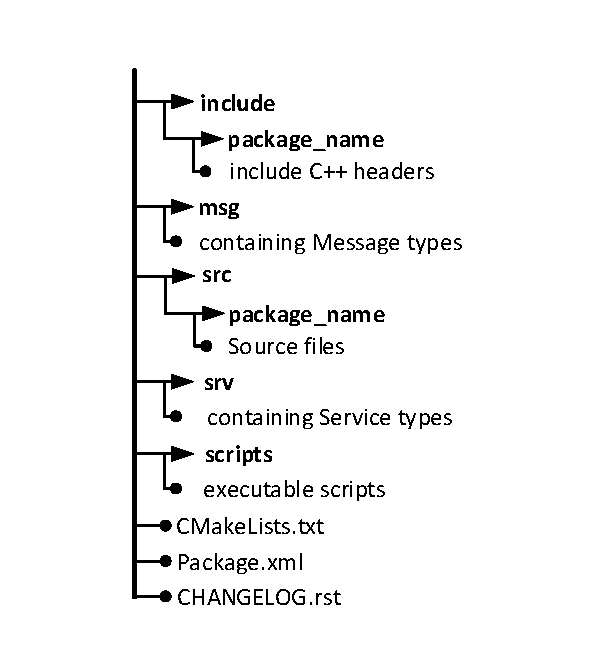
\includegraphics[width=0.6\textwidth]{structure.pdf}
\end{figure}
% \begin{itemize}
 %\item include/package\_name: include C++ headers 
 %\item msg/: containing Message types
 %\item src/package\_name/:  Source files
 %\item srv/: containing Service types
 %\item scripts/: executable scripts
 %\item CMakeLists.txt:  CMake build file
 %\item package.xml 
 %\item CHANGELOG.rst
 %\end{itemize}
\end{frame}
%----------------------------------------------------------------------------------------
%\section{Concepts}
%----------------------------------------------------------------------------------------
\begin{frame}{Setup the built environment}
 \textbf{Creating a workspace}
 %\begin{itemize}
 %\item \$ source /opt/ros/indigo/setup.bash
 %\item \$ mkdir -p \textasciitilde/catkin\_ws/src
 %\item \$ cd \textasciitilde/catkin\_ws/src
 %\item \$ catkin\_init\_workspace
 %\end{itemize}
 \lstinputlisting[frame=single, basicstyle=\footnotesize\ttfamily, language=C]{setup_the_build_environment.txt}
 \textbf{Build empty project}
% \begin{itemize}
% \item \$ cd \textasciitilde/catkin\_ws/
% \item \$ catkin\_make
% \end{itemize}
  \lstinputlisting[frame=single, basicstyle=\footnotesize\ttfamily, language=C]{build_empty_project.txt}

 \textbf{Environment-Variables loaded?}
 %\begin{itemize}
 %\item \$ source devel/setup.bash
 %\item \$ echo \$ROS\_PACKAGE\_PATH
 %\item /home/youruser/catkin\_ws/src:/opt/ros/indigo/share: /opt/ros/indigo/stacks
 %\end{itemize}
  \lstinputlisting[frame=single, basicstyle=\footnotesize\ttfamily, language=C]{environment_variables_loaded.txt}

\end{frame}
%----------------------------------------------------------------------------------------
%----------------------------------------------------------------------------------------
\begin{frame}{Create and Build a ROS Package}
 \textbf{Create a new package called ’beginner\_tutorials’ which
depends on std\_msgs, roscpp, and rospy
}
 %\begin{itemize}
 %\item \$ catkin\_create\_pkg beginner\_tutorials std\_msgs rospy roscpp
 %\end{itemize}
   \lstinputlisting[frame=single, basicstyle=\footnotesize\ttfamily, language=C]{crate_new_package.txt}

 \textbf{Build a package}
 %\begin{itemize}
 %\item \$ cd \textasciitilde/catkin\_ws/
 %\item \$ catkin\_make
 %\end{itemize}
    \lstinputlisting[frame=single, basicstyle=\footnotesize\ttfamily, language=C]{build_a_package.txt}
\end{frame}
%----------------------------------------------------------------------------------------
%----------------------------------------------------------------------------------------
\begin{frame}{Eclipse and ROS}
 \textbf{Creating the Eclipse project files}
 
 \lstinputlisting[frame=single, basicstyle=\footnotesize\ttfamily, language=C]{creating_the_eclipse_project_files.txt}
 
 \textbf{Importing the project into Eclipse}
 \begin{itemize}
 \item Start Eclipse, select File  --\textgreater  Import. Select  Existing projects into workspace, hit next, then browse for your package's directory (select root directory). Do NOT select Copy projects into workspace. Then finish.
 \end{itemize}
\end{frame}
%----------------------------------------------------------------------------------------
%----------------------------------------------------------------------------------------
\begin{frame}{Eclipse and ROS}

 \textbf{Importing the project into Eclipse}

\begin{figure}[htb]
    \centering
    \begin{minipage}{0.45\linewidth}
        \centering
        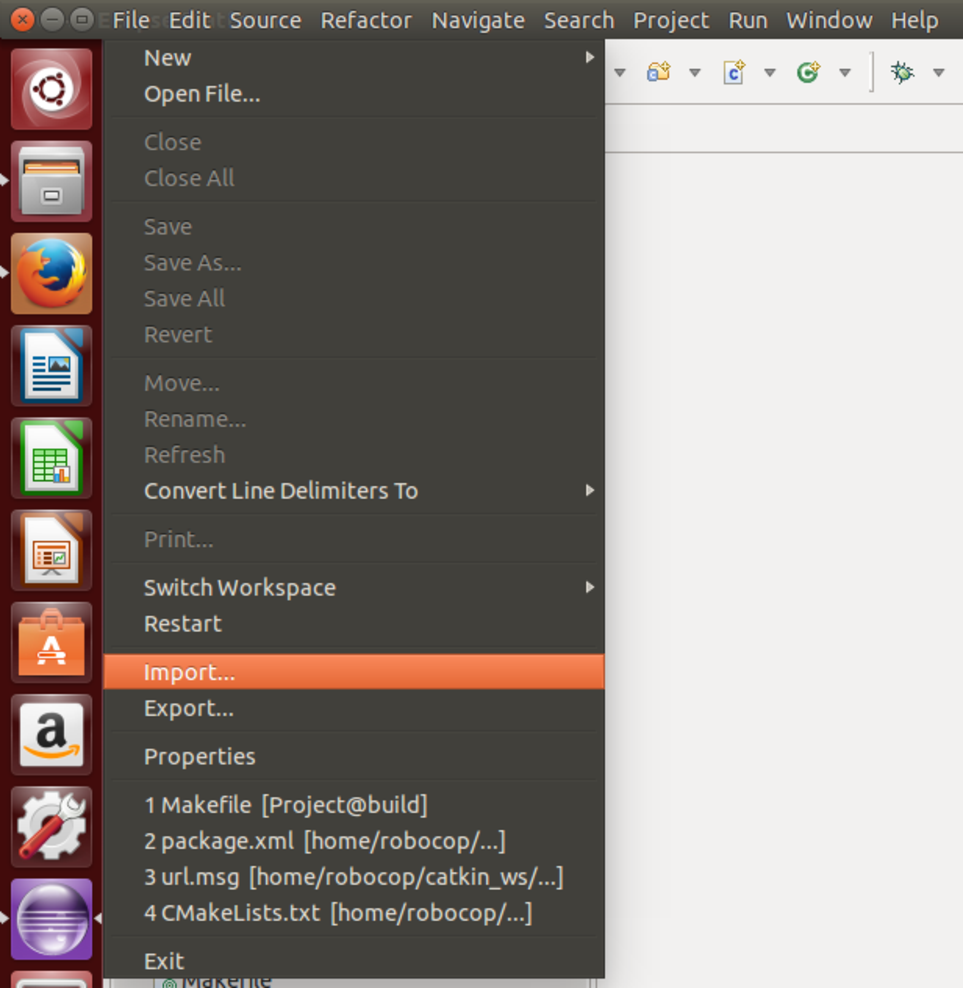
\includegraphics[scale=0.3]{import.pdf}
    \end{minipage}
    %\hfill
    \begin{minipage}{0.45\linewidth}
        \centering
        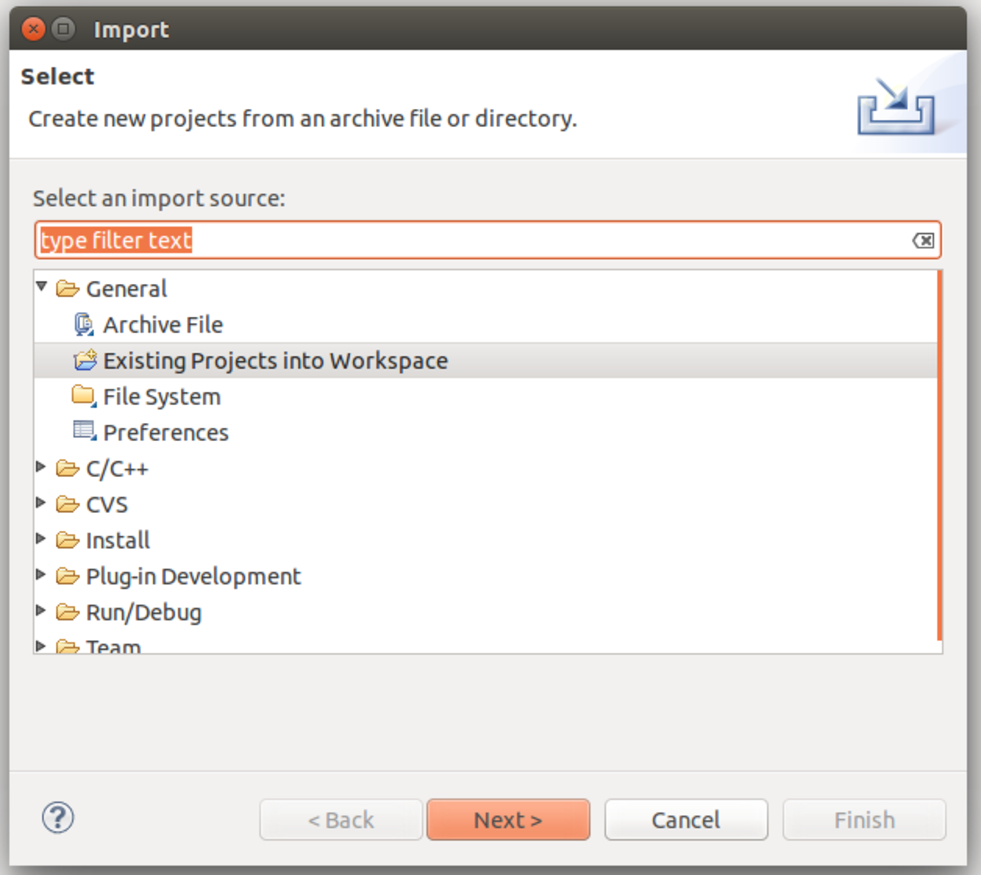
\includegraphics[scale=0.35]{select.pdf}
    \end{minipage}
        \caption{Start Eclipse, select File  --\textgreater  Import. Select Existing projects into workspace, hit next.}
\end{figure}

\end{frame}
%----------------------------------------------------------------------------------------
%----------------------------------------------------------------------------------------
\begin{frame}{Eclipse and ROS}

\begin{figure}
	\centering
  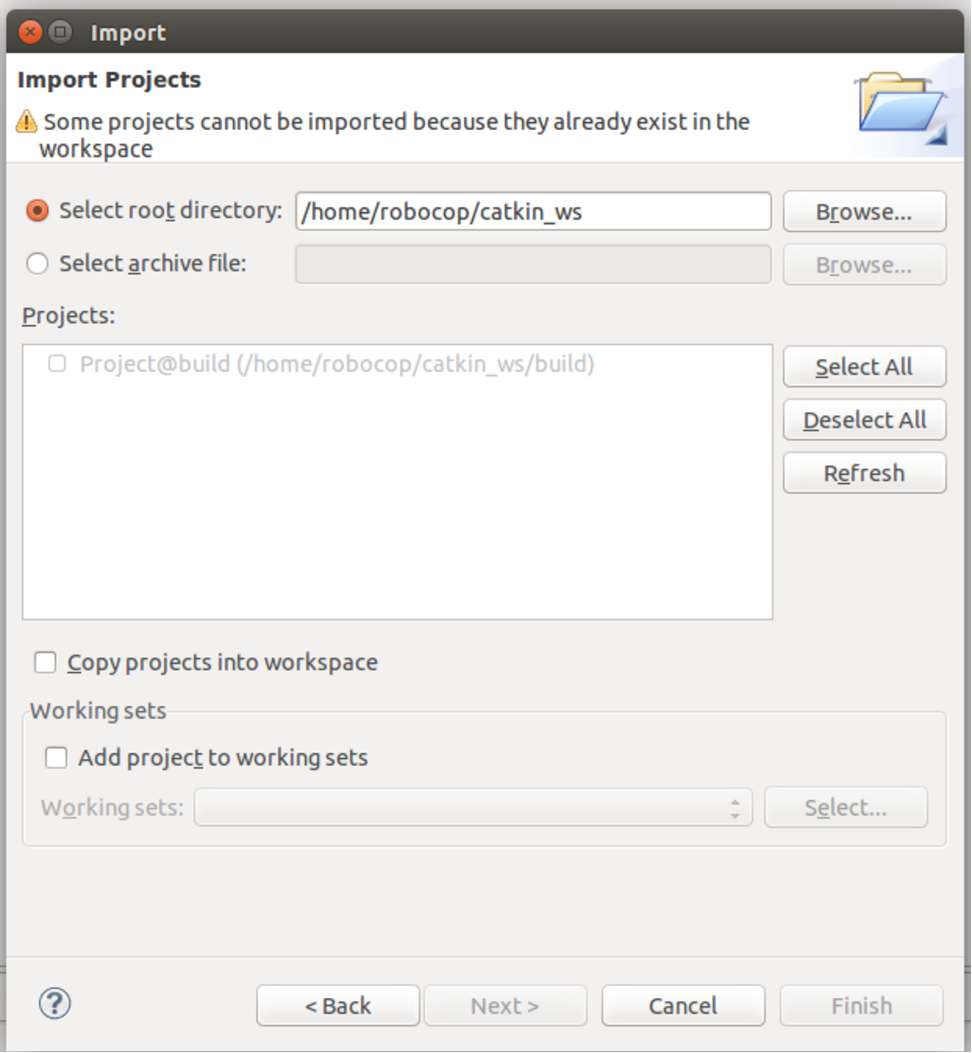
\includegraphics[width=0.35\textwidth]{file.pdf}
	\caption{Browse for your package's directory (select root directory). Do NOT select Copy projects into workspace. Then finish.}
	\label{fig1}
\end{figure}

\end{frame}
%----------------------------------------------------------------------------------------
%----------------------------------------------------------------------------------------
%\begin{frame}[allowframebreaks]{References}
%\scriptsize{\bibliographystyle{ieeetr}}
%\bibliography{references} %bibtex file name without .bib extension
%\end{frame}
%----------------------------------------------------------------------------------------
\begin{frame}
\Huge{\centerline{The End}}
\end{frame}
%----------------------------------------------------------------------------------------
\end{document} 
%----------------------------------------------------------------------------------------